\begin{sagesilent}
import matplotlib.pyplot as plt
import numpy as np

d = load("sobj/oscilloscopio-c2.sobj", verbose=False)
d.sort()

plt.clf()
plt.ylim(ymin=3, ymax=15)
plt.title("Grafico 1")
plt.xlabel("Frequenza (Hz)")
plt.ylabel("Corrente (mA)")
plt.grid(True, which='both')
plt.loglog(d['frequenza_hz'], d['i_ma'], '.r')
plt.savefig("grafici/C2-1.png", dpi=300)

plt.clf()
plt.ylim(ymin=0.3, ymax=1.5)
plt.grid(True, which='both')
plt.title("Impedenze")
plt.loglog(d['frequenza_hz'], d['valore_mu']/d['v_rms'], '.r')
plt.savefig("grafici/C2-2.png", dpi=300)
\end{sagesilent}


\chapter{C2}

\section{Risposta in frequenza del multimetro}
\begin{center}
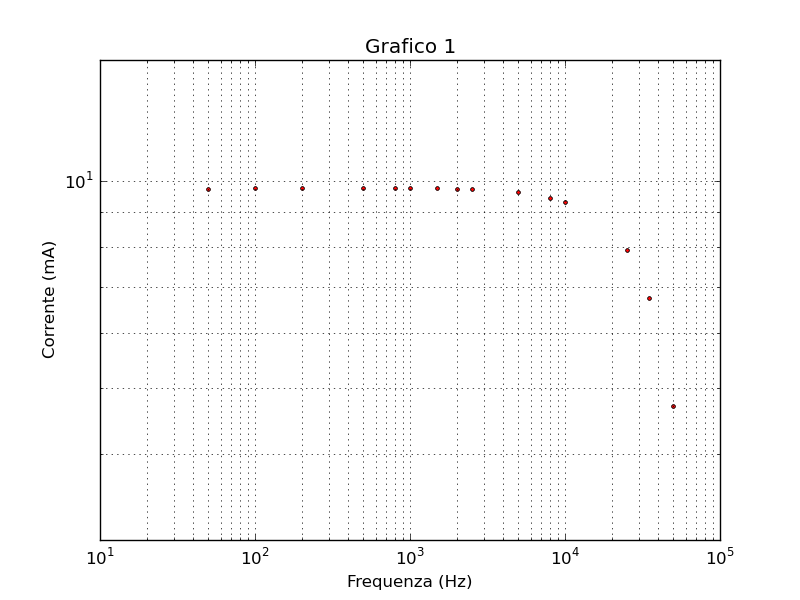
\includegraphics[scale=0.75]{grafici/C2-1.png} 
\end{center}

\section{Misura di impedenze ignote}
\begin{center}
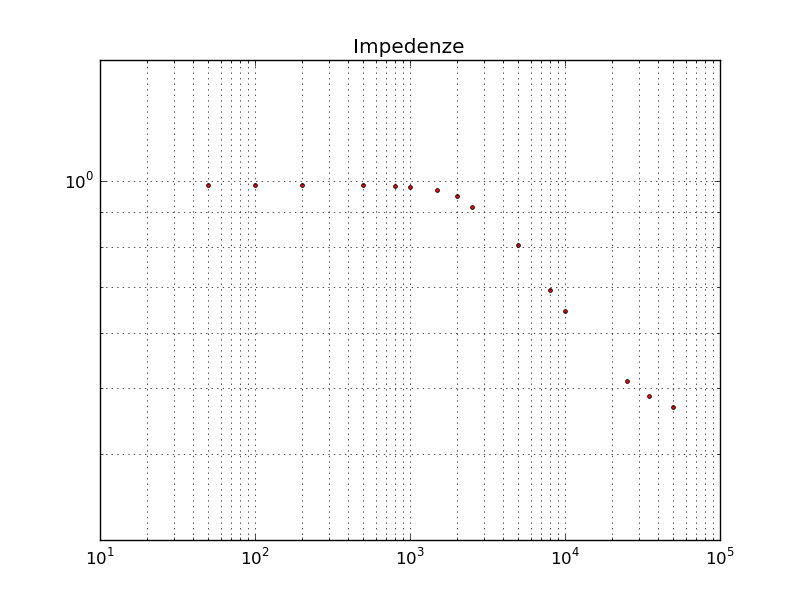
\includegraphics[scale=0.75]{grafici/C2-2.png} 
\end{center}

L'obiettivo del nostro esperimento è misurare la velocità della luce $c$.

L'apparato di misurazione consiste principalmente in:

\section{Analisi dati}

\section{Allegato: dati}
\begin{sagesilent}
def stampa_dati(wa, header):
  s = r"\begin{tabular}{c*{" + "%d" % (len(wa.dtype)-1)
  s += r"}{|c}}"
  s += "%s \\\\" % (header)
  s += r"\midrule"
  for i in range(0, len(wa)):
    a = ["%s" %x for x in d[i]]
    s += "%s \\\\" % join(a, "&")
  s += r"\end{tabular}"
  return s
\end{sagesilent}

\begin{center}

\sagestr{stampa_dati(d, r"Frequenza (Hz) & I (mA) & Valore mu & $V_{rms}$ (V)")}
\end{center}

